\subsection{Interações entre Módulos Grasews}\label{4-grasews-interacoes-modulos}

A \figurename~\ref{fig:grasews-architecture-simplified} apresenta uma visão geral das principais interações existentes entre os módulos Grasews. Uma seta preta e sólida representa as interações de um usuário com a aplicação. Uma linha azul, sólida e com setas sólidas nas duas extremidades representa interações entre os módulos utilizando objetos, i.e., instâncias de classes conforme a programação orientada a objetos. Uma linha rosa e tracejada representa injeções de dependências. Uma linha verde e tracejada representa implementações de interfaces de desenvolvimento. A extremidade com a seta verde e vazia indica a definição das interfaces contidas em \texttt{Grasews.Domain}, enquanto que a extremidade com o círculo verde e sólido indica um módulo que implementa uma interface definida em \texttt{Grasews.Domain}. Uma seta vermelha e tracejada indica interações realizadas por meio do protocolo HTTP entre os módulos da aplicação. Por fim, uma seta laranja e tracejada representa eventos assíncronos. A extremidade com o círculo laranja e vazio representa a origem dos eventos assíncronos, enquanto que a extremidade com a seta laranja e vazia indica o módulo onde os eventos assíncronos são notificados.

\begin{figure}[h]
    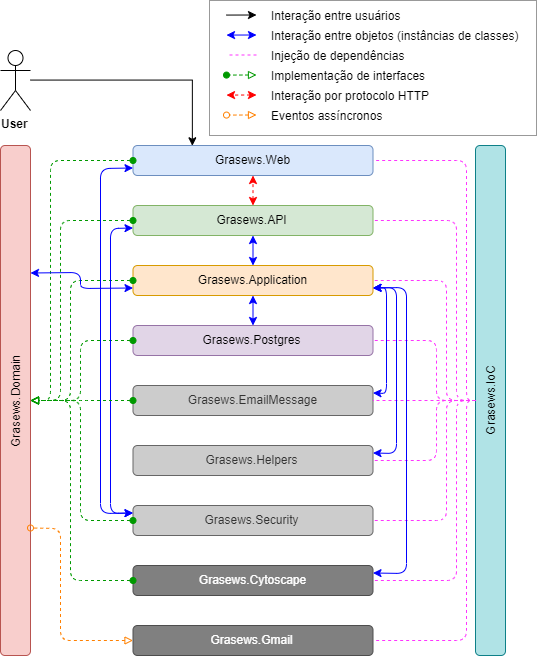
\includegraphics[scale=0.55]{4-grasews/imagens/grasews-architecture-simplified.png}
    \centering
    \caption[Arquitetura da ferramenta Grasews]{\textbf{Arquitetura da ferramenta Grasews.}}
    \label{fig:grasews-architecture-simplified}
\end{figure}

De forma resumida e simplificada, o fluxo da aplicação segue da seguinte forma: O usuário interage com o módulo \texttt{Grasews.Web}, o qual se comunica com \texttt{Grasews.API} por meio de requisições HTTP. Tanto \texttt{Grasews.Web} quanto \texttt{Grasews.API} utilizam funcionalidades providas por objetos de \texttt{Grasews.Security}. \texttt{Grasews.API} consome serviços providos por \texttt{Grasews.Application}, o qual orquestra o fluxo de trabalho conforme as regras de negócio da aplicação. Neste sentido, \texttt{Grasews.Application} é responsável por manipular objetos das entidades de domínio da aplicação juntamente com funcionalidades de apoio providas por \texttt{Grasews.Helpers}. Adicionalmente, \texttt{Grasews.Application} utiliza funcionalidades providas por \texttt{Grasews.Cytoscape}, para a manipulação de elementos do grafo, e funcionalidades providas por \texttt{Grasews.EmailMessage}, para a construção de mensagens de \textit{e-mail}. Juntamente com \texttt{Grasews.Gmail}, \texttt{Grasews.Application} invoca um evento assíncrono de \texttt{Grasews.Domain} para que a mensagem de \textit{e-mail}, previamente construída por \texttt{Grasews.EmailMessage}, seja enviada para um usuário. \texttt{Grasews.IoC} provê a injeção de dependências para todos os demais módulos da arquitetura.